\section{Blockchain applications}

Now that we've understood the principles of blockchains, we may wonder what are the main uses nowadays.

\paragraph{Why people use blockchains instead of other security methods?}

We can suggest a few reasons to answer this question (see \cite{blockchainPros}) :

\begin{itemize}
  \item Blockchains are fast, secure and transparent. Moreover, history has proven its robustness since no attacks resulted from a weakness inside the blockchain itself.
  \item In general, people have a great opinion of it: 84\% think it provided more security than other methods.
  \item One can estimate around 70\% cost savings on business operation and 30 - 50 \% on compliance.
\end{itemize}

\paragraph{What are the main blockchain applications?}

In the few last years, we've seen a lot of new blockchains being launched in different fields. We can have a look at some of them (see \cite{usesBlockchain})\newline

\begin{figure}[ht]
\centering
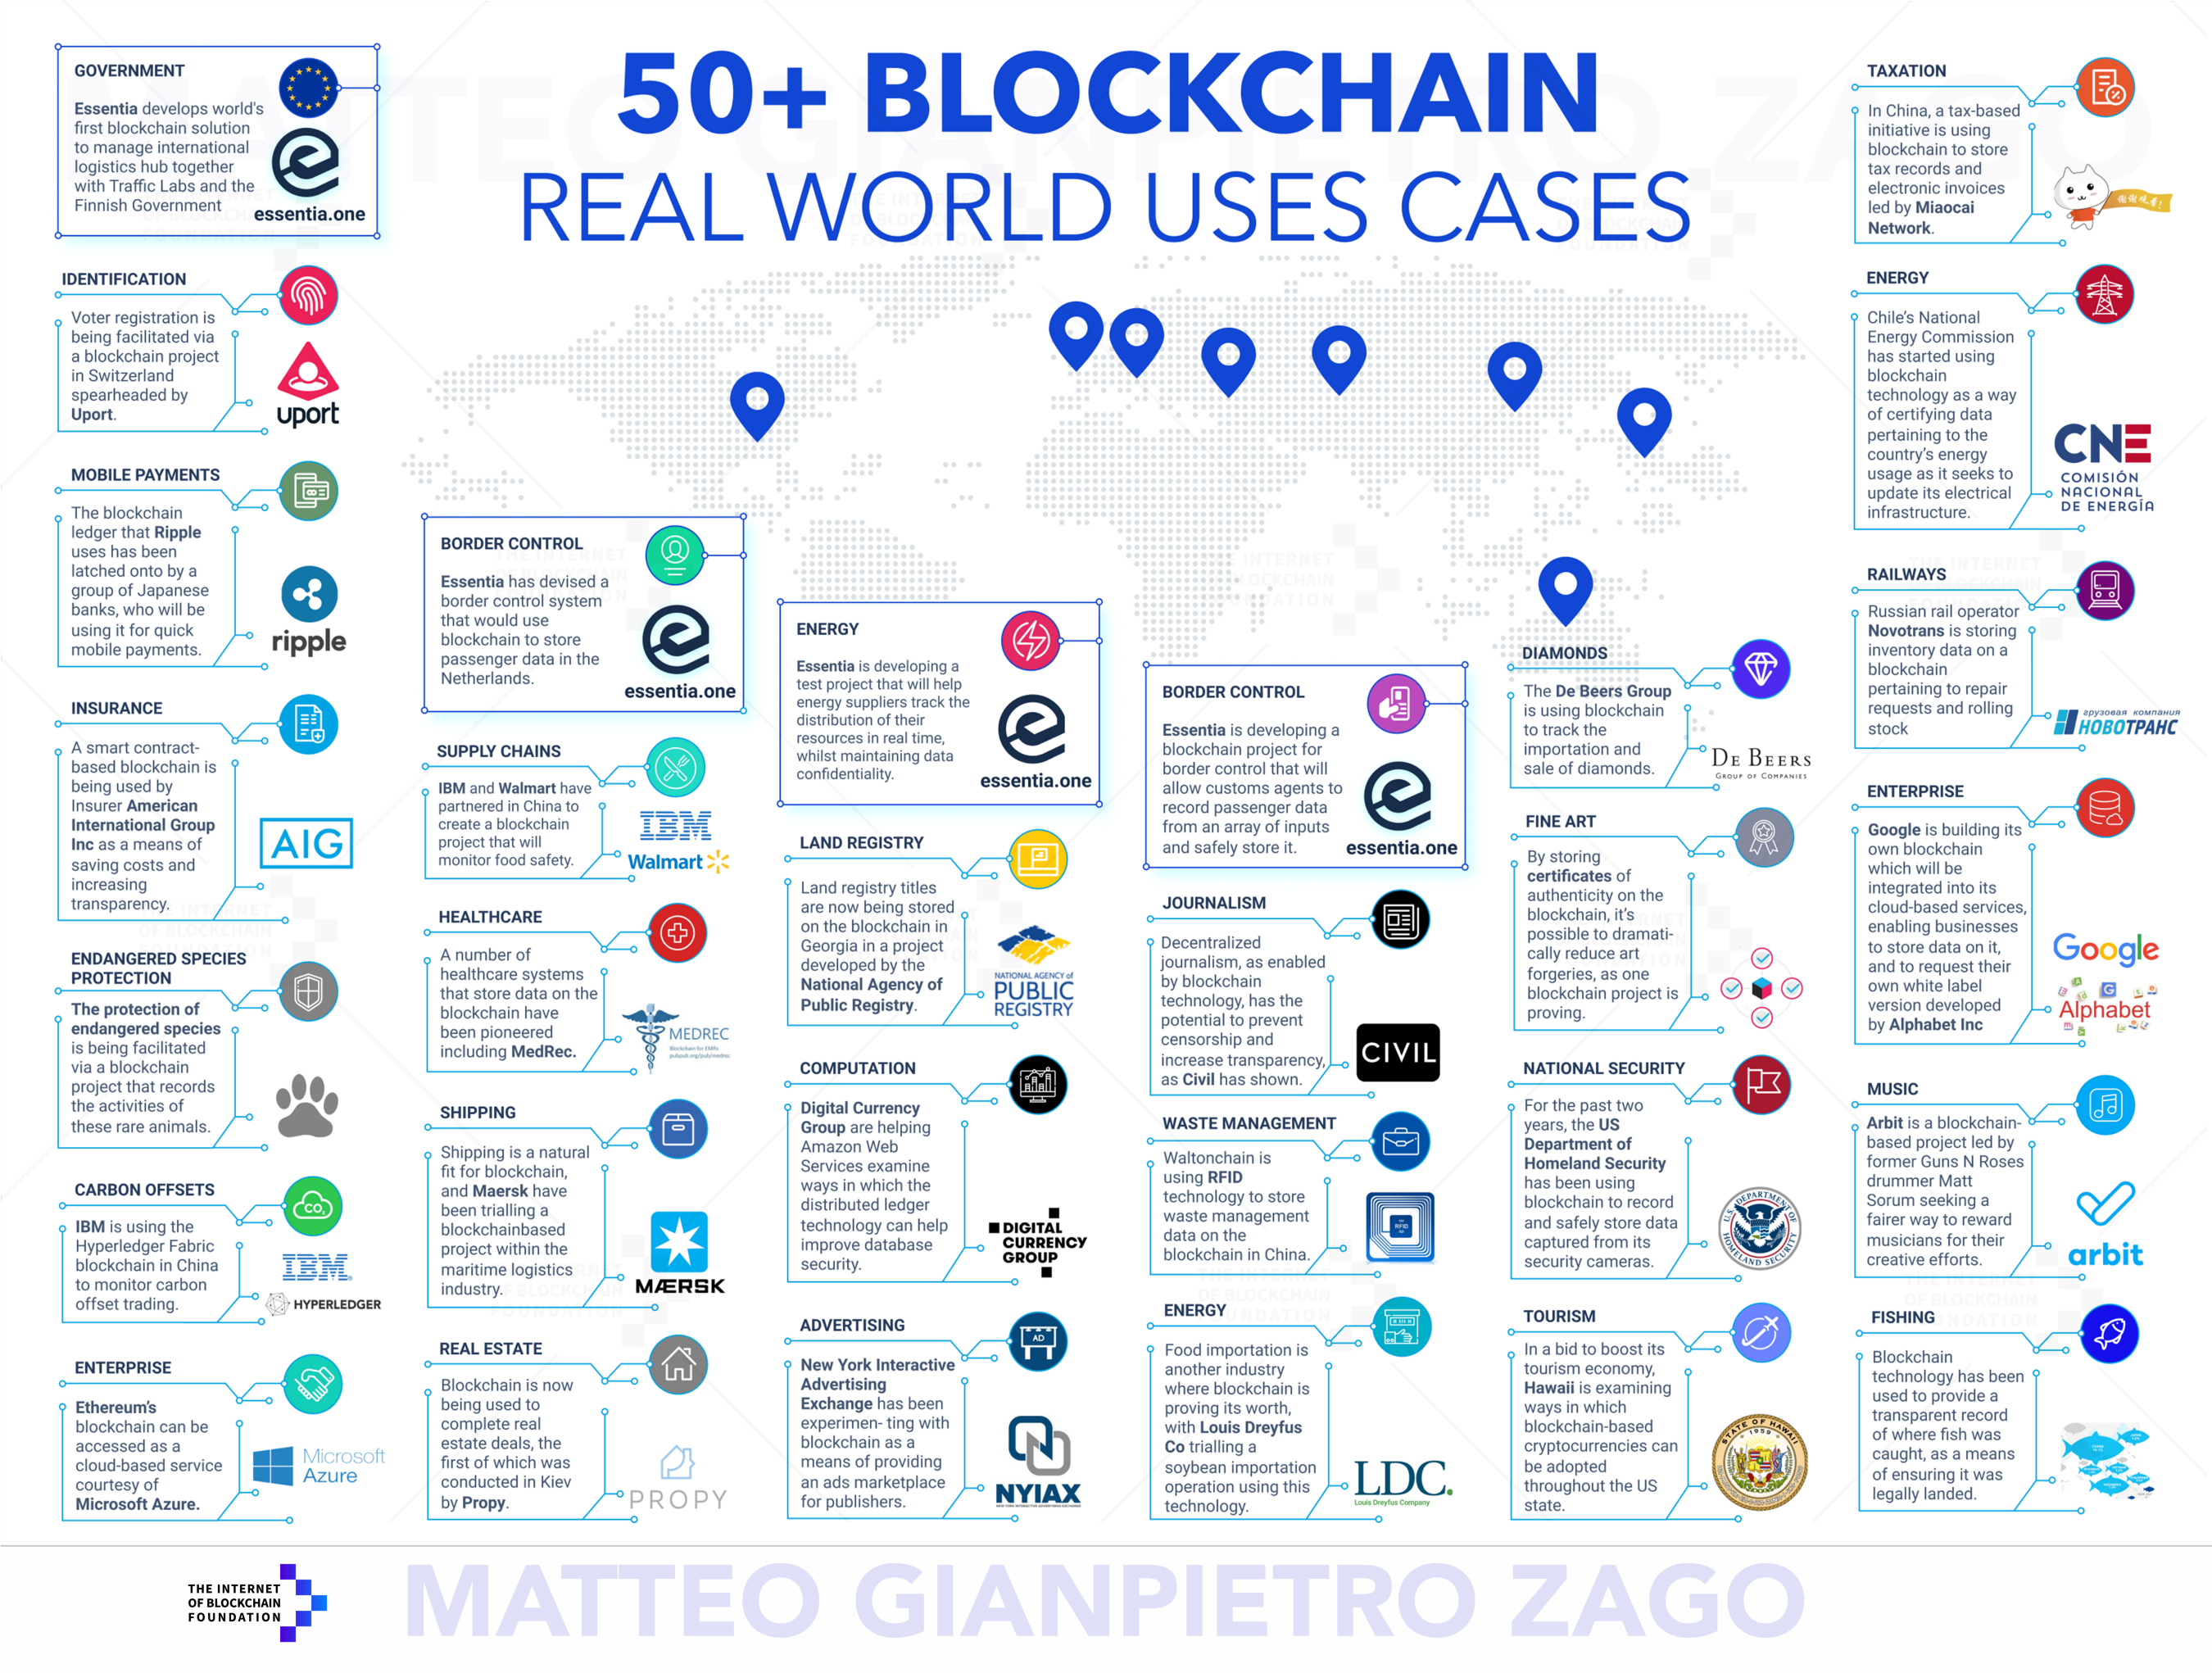
\includegraphics[width=10cm]{Figures/blockchainUses}
\caption{Blockchain uses in the world (see \href{https://medium.com/@matteozago/50-examples-of-how-blockchains-are-taking-over-the-world-4276bf488a4b}{Link to medium.com})}
\end{figure}
\medskip

We see that blockchains may be used by governments for taxation and border controls, in the energy field and social field for insurance and healthcare. \newline

We can take the example of Uport who created a platform based on Ethereum blockchain to register residents' ID (see \cite{uport}). They collaborated with the city of Zug (Switzerland) to allow residents to access eServices like online voting. \newline

The first step for a Zug citizen is to create his digital identity on the Uport platform. He will have to fill a form with his data and to visit one of the Zug offices in person to cross-check his digital identity. Then, he will get his credentials to access Zug eServices. \newline

The city of Zug planned to develop its service of online voting in Spring 2018 using this new technology.

Eventually, blockchains could facilitate a lot the interactions between people and governments.
